%%%%%%%%%%%%%%%%%%%%%%%%%%%%%%%%%%%%%%%
\documentclass[uplatex,a4paper,9pt]{bxjsarticle}
\usepackage{amsmath}
\usepackage{newtxmath,newtxtext}
\usepackage{type1cm}
\usepackage[dvipdfmx]{graphicx}
\usepackage{subfigure}
\usepackage{tacksyuron}
\usepackage{cite}
\usepackage{url}
%
\newcommand{\ignore}[1]{}
\newcommand{\bs}{\boldsymbol}
%
\setcounter{topnumber}{5}%ページ上部の図表は 5 個まで
\def\topfraction{1.00}%ページの上 1.00 まで図表で占めて可
\setcounter{bottomnumber}{5}%ページ下部の図表は 5 個まで
\def\bottomfraction{1.00}%ページの下 1.00 まで図表で占めて可
\setcounter{totalnumber}{10}%ページあたりの図表は 10 個まで
\def\textfraction{0.04}%ページうち本文が占める割合の下限
\def\floatpagefraction{0.7}%図表だけのページは少なくともこれだけを
%%%%%%%%%%%%%%%%%%%%%%%%%%%%%%%%%%%%%%%

\tackTitle{\LARGE 卒業研究発表会向け概要\LaTeX スタイルファイルの使い
方}
\tackAuthor{G082002020}{拓殖 太郎}{渡邊}{修}{教授}

\begin{document}
\mktitle
\section{はじめに}
本稿では\LaTeX の基本的な使い方と,卒業研究ならびに修論の発表会用概要原稿作成の
ための\LaTeX スタイルファイル(\verb|tacksyuron.sty|)の使い方を解説する.
\section{タイトルおよび著者}
原稿のタイトルと著者名や学籍番号の記述は,本文開始前の部分(プリアンブル
)に以下のコマンドを記述する\footnote{ここで述べるのは tacksyuron.sty 独自
  の方法であり,\LaTeX の一般的な方法とは異なる.}.以下,バックスラッシュ
  (\verb|\|)は,Windows上では¥記号(\verb|¥|)を入力することに注意.
\begin{verbatim}
\tackTitle{原稿タイトル}
\tackAuthor{学籍番号}{著者氏名}{教員の姓}{教員の名}{教員の職位}
\end{verbatim}
以上のコマンドをプリアンブルに記述しておき,ドキュメント開始の最初の行に
\verb|\mktitle|
とコマンドを書いておくと,タイトルと著者欄が出力される.
\section{数式について}
\LaTeX では美しい数式を表示することができる.
簡単なものだと$y=ax+b$のように行中に置くこともできるし,複雑な数式は
\begin{align}
X_k &= \sum_{n=0}^{N-1}x_n e^{-j\frac{2\pi kn}{N}} \label{fdft}\\
x_n &= \frac{1}{N}\sum_{k=0}^{N-1}X_k e^{j\frac{2\pi kn}{N}} \label{idft}
\end{align}
のように別行立てにする.別行立てにすると式番号が自動的に付き,ラベルを記
述しておけばあとで参照することができる.式
(\ref{fdft})は離散フーリエ変換,式(\ref{idft})は離散フーリエ逆変換の定義
式である.
\section{図表}
\begin{itemize}
\item 図はPDF形式で作成しておく.作成方法は後述.
\item 表はソースファイル中に記述する.
\end{itemize}
図番号は自動的に付く.
\begin{figure}[b]
\centering
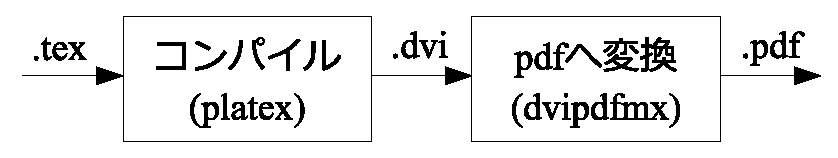
\includegraphics[width=0.8\columnwidth]{./testfig.eps}
\caption{\TeX 文書作成の流れ}
\label{fig1}
\end{figure}
\subsection{図の挿入例}
figure環境を用いて本文に挿入する.結果を図\ref{fig1}に示す.オプション\verb|[!htbp]|を組み合わせて
図の配置をある程度決めることが出来る.各オプションの意味は以下のとおり.
\begin{description}
\item[\tt h] 「ここ」(here),あまり使わない
\item[\tt t] 「ページ上部」(top)
\item[\tt b] 「ページ下部」(bottom)
\item[\tt p]  別ページ
\item[\tt !] 「強制」あまり使わない
\end{description}
\subsection{表の挿入例}
table環境を用いて本文に挿入する.結果を表\ref{tab1}に示す.figure環境と
同じく,オプション\verb|[!htbp]|を組み合わせて配置をある程度決めることが出来る.
\begin{table}[tb]
\centering
\caption{仕入れる果物の数量および価格}
\label{tab1}
{\small
\begin{tabular}{c|c|c|c}\hline
品名 & 単価 & 個数 & 金額 \\ \hline\hline
りんご & 100 & 5 & 500 \\ \hline
バナナ & 50 & 50 & 2500 \\ \hline
\end{tabular}
}
\end{table}
\subsection{図の作成方法}
印刷が想定される文書向けに図を作成する場合,ベクター形式で作成するのが望
ましい.Windowsの\LaTeX で容易に用いることができるのはEPS(Encapsulated
PostScript)形式である(LinuxやmacOSではPDF形式の図を容易に取り扱うことができる).Microsoft OfficeにはEPS形式への出力機能がないため,フリーのオフィ
スソフトであるLibre Officeを用いる.Libre Officeを用いた図やグラフの作成
方法についてはサイト\cite{labEditorTips}を参照のこと.なお,Libre Office
はExcelで作成した.xls,.xlsxファイルを読み込むことができる.
\section{参考文献の追加}
参考文献はソースファイルの最後にまとめて記述しておく.
記述した順に番号が自動的に追加される.例えば,文献\cite{BrainBook}や
文献\cite{EBCOTpaper},となる.さらに,文献\cite{BrainBook, EBCOTpaper}など
のようにすることもできる.

\section{おわりに}
\LaTeX に関する詳しい使い方は
文献\cite{okumura}が最も分かりやすく,詳しい.
インターネットでは,\cite{TeXWiki,latexComSheet}が参考になる.
図表の作成方法や,\LaTeX 文書への挿入の方法は\cite{labEditorTips}が役に
立つ.
\section*{謝辞}
本研究を進めるにあたりご指導頂いた○○教授,助手の○○先生,並
びに○○研究室諸氏に感謝する.
\footnotesize
\begin{thebibliography}{9}
\bibitem{okumura} 奥村晴彦 ``[改訂第4版] \LaTeXe 美文書作成入門'',技術評論社,2007年.
\bibitem{TeXWiki} ``\TeX Wiki'',\url{http://oku.edu.mie-u.ac.jp/~okumura/texwiki/}
\bibitem{latexComSheet} ``LaTeX コマンドシート'', \url{http://www002.upp.so-net.ne.jp/latex/index.html}
\bibitem{labEditorTips} \url{http://www.labeditor.com/lab_tips.html}
\bibitem{BrainBook} 榊原学,吉岡亨 ``システムとしての脳'',共立出版社,2003年.
\bibitem{EBCOTpaper} D.\ Taubman, ``High Performance Scalable Image Compression with EBCOT,'' IEEE Trans.\ Image Processing, vol.9, no.7, pp.1158--1170, Jul.\ 2000.
\end{thebibliography}
\end{document}